\documentclass[12pt,a4paper]{article}
\usepackage[bottom=2.5cm,top=3.5cm]{geometry}
%\usepackage{ngerman}
\usepackage[utf8]{inputenc}
\usepackage[T1]{fontenc}
\usepackage{microtype}
\usepackage{graphicx}
\usepackage{ae}
\usepackage{amssymb}
\usepackage{amsmath}
\usepackage{amsthm}
\usepackage[margin=10pt,font=small,labelfont=bf]{caption}
%\usepackage[pdftex]{graphicx}
\usepackage{listings}
%\linespread{1.25}
\setlength{\parindent}{0pt}

\usepackage{fancyhdr}
\usepackage[
  	pdfstartview=FitH,   
  	pdffitwindow=true,
	pdftitle = "Optimisation SS10 UdS", % Sets the document information Title field
    pdfauthor = "Adrian Neumann and Sebastion Steenbruck", %Sets the document information Author field
  	colorlinks,
  	linkcolor=black,
  	anchorcolor=black,
  	citecolor=black,
  	urlcolor=black
]{hyperref}

\pagestyle{fancy}
\cfoot{\thepage}
\rfoot{
\includegraphics{./images/by-nc-sa.pdf}}
\fancyhead{}
\lfoot{}
\renewcommand{\footrulewidth}{0.4pt}
\renewcommand{\headrulewidth}{0pt}
\newcommand{\N}[0]{\mathbb{N}}
\newcommand{\Z}[0]{\mathbb{Z}}
\newcommand{\Q}[0]{\mathbb{Q}}
\newcommand{\R}[0]{\mathbb{R}}
\newcommand{\C}[0]{\mathbb{C}}
\newcommand{\im}[0]{\mathit{i}}
\newcommand{\kthings}[2]{{#1}_1,\ldots,{#1}_{#2}}
\newcommand{\nthings}[1]{\kthings{#1}{n}}
\newcommand{\norm}[1]{|\!|#1|\!|}
\newcommand{\rank}{\mbox{rank }}
\renewcommand{\bar}{\overline}
\newcommand{\trans}[1]{{#1}^\text{\upshape \sffamily T}}
\newtheoremstyle{leplain} %name
    {3pt} %above
    {3pt} %below
    {} %body font
    {} %indent
    {\bfseries} %head font
    {:} %punctuation after head
    {0.5em} %space after head
    {} %head spec
\title{Optimisation}
\author{Adrian Neumann \\ {\small \texttt{adrian\_neumann@gmx.de}} \and Sebastian Steenbuck \\ {\small\texttt{sebastian@steenbuck.org}}}


\date{}\begin{document}
\lstdefinelanguage{pseudocode}{
    morekeywords = {repeat, until, if, while, for},
    sensitive = false,
    morecomment=[1]{//},
    morecomment=[s]{/*}{*/},
}
\lstset{language=pseudocode, basicstyle=\sffamily\small\slshape, commentstyle=\slshape\sffamily, keywordstyle=\upshape\bfseries, breaklines=true, mathescape=true, tabsize=2}


\theoremstyle{definition}
\newtheorem{Def}{Definition}[section]

\theoremstyle{leplain}
\newtheorem{Ex}{Example}[section]
\newtheorem{pr}{Proof}[section]
\newtheorem{cor}{Corollary}[section]

\theoremstyle{theorem}
\newtheorem{thm}{Theorem}[section]



\maketitle
\thispagestyle{fancy}

\marginpar{Tutorial}
\section*{Tutorial}
Some definitions from linear algebra, which were repeated in the tutorial.

Linear algebra was originally developed from geometry but has come to be an important foundation in mathematics. To keep things simple we'll restrict ourselves to $\R^n$ although other structures could be used.

\begin{Def}[Vector space] 
A vector space (for our purposes) is a set of points $$\R^n=\{(x_1,x_2,...,x_n)|x_i \in \R\}$$ that is closed under linear combination.
\end{Def}

\begin{Def}[Linear Combination] 
A linear combination $w$ is defined as the sum of all the vectors in a set $V$ multiplied with some scalars $\lambda$.
$$w=\sum_{i \in V}{\lambda_i v_i} \qquad \lambda_i \in \R,v_i\in V$$ 
\end{Def}  

As infinite sets are hard to describe we're looking for a \emph{Basis} $S$. Which is a subset of $\R^n$ such that every vector in $\R^n$ can be represented as a unique linear combination of the elements of $S$.

The vectors in a basis must be \emph{linearly independent}, that is none of them can be written as a linear combination of the others. The standard basis for $\R^n$ is the set of $n$-dimensional unit vectors.

\[\left\{\begin{pmatrix}1\\0\\\vdots\\0\end{pmatrix},\begin{pmatrix}0\\1\\\vdots\\0\end{pmatrix},\ldots,\begin{pmatrix}0\\\vdots\\0\\1\end{pmatrix}\right\}\]


\begin{thm} 
Every basis of a vector space $\R^n$ has the same number of elements, which is $n$. 
\end{thm}

This follows for example from \href{http://en.wikipedia.org/wiki/Steinitz_exchange_lemma}{Steinitz exchange lemma}.

\begin{Def}[Subspace]
 A subspace $V$ of a vector space $\R^n$ is spanned by a subset of the a basis of $R^n$. Examples of a subspace in 2D are all the lines going through the point $(0,0) \in \R^2$.
\end{Def}

To get a notion of angle between vectors we introduce the dot product (in euclidean spaces also called: inner product). It is defined as

\[\langle x,y\rangle  = \sum x_iy_i\]

It is related to the law of cosines in two dimensions ($c^2 = a^2+b^2-2ab\cos \gamma$) like this:

\begin{minipage}[hbt]{0.5\linewidth}
\begin{align*}
\norm{\vec c}^2 &= \norm{\vec a}^2 + \norm{\vec b}^2 -2\norm{\vec a}\norm{\vec b}\cos \gamma\\
\norm{a-b}^2 &= \norm{\vec a}^2 + \norm{\vec b}^2 -2\norm{\vec a}\norm{\vec b}\cos \gamma\\
\norm{a}^2-2\langle a,b\rangle +\norm{b}^2 &= \norm{\vec a}^2 + \norm{\vec b}^2 -2\norm{\vec a}\norm{\vec b}\cos \gamma\\
\frac{\langle a,b\rangle }{\norm{a}\norm{b}} = \cos \gamma
\end{align*}
\end{minipage}
\hfill
\begin{minipage}[hbt]{0.3\linewidth}
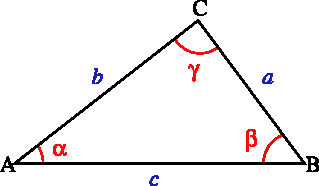
\includegraphics[scale=0.8]{./images/Triangle_with_notations_2.pdf}
\end{minipage}

\bigskip
(Here $\norm{a}$ denotes the norm: $\sqrt{\sum a_i^2} = \sqrt{\langle a,a\rangle }$). The dot product is $0$ if and only if the vectors are orthogonal to each other.

Now that we have defined vector spaces we want to study some linear transformations on them. Since vector spaces are closed under linear combination we'd like to have our transformation preserve that structure.

\begin{Def}[Linear Transformation] A linear transformation is (for our purposes) a mapping $T : \R^n \rightarrow \R^m$ with the following properties:

\begin{enumerate}
\item $T(\lambda w) = \lambda T(w)$
\item $T(v+w) = T(v)+T(w)$
\end{enumerate}
\end{Def}

Prominent examples for linear transformations are rotations and reflections around the origin. Note that if $T(\vec 0)\neq 0$ you automatically know that it's not a linear transformation.

If we use a standard basis for our vector space we can easily represent linear transformations by their effects on the basis. Just map every basis vector to its image and write the results in a matrix. 

\begin{Ex}[Reflection] Suppose we want to reflect every vector in $\R^2$ at the x-axis. If we use the standard base $V = \{(1,0),(0,1)\}$ and compute its reflection $V'=\{(1,0),(0,-1)\}$ we get the matrix

\[R = \begin{pmatrix}
1 & 0 \\
0 & -1
\end{pmatrix}\]

Multiplying a vector with that matrix we get its reflection. Just in case: Matrix multiplication

\[\begin{pmatrix}
a_{11} & a_{12} & \ldots & a_{1n}\\
a_{21} & a_{22} & \ldots & a_{2n}\\
\vdots \\
a_{m1} & a_{m2} & \ldots & a_{mn}
\end{pmatrix} * \begin{pmatrix}x_1\\x_2\\\vdots\\x_n\end{pmatrix} =\begin{pmatrix} \sum_{i=1}^n a_{1i}x_i\\ \sum_{i=1}^n a_{2i}x_i\\\vdots\\\sum_{i=1}^n a_{mi}x_i\end{pmatrix}\]

\end{Ex}

Note that for two transformations $f,g$ and their matrices $A,B$ we have
\[\forall \vec v:\ (f\circ g)(v) = (AB)v\]

\begin{Def}[Kernel of a matrix] 
 The kernel of a matrix $A$ is the set of all vectors $x$ with
$$Ax=0$$
\end{Def}

\begin{Def}[Rank of a matrix]
 The rank of a matrix $A$ is the number of linearly independent columns or rows of $A$. The column and row rank is always the same. In other words the row (column) rank is the dimension of the subspace spanned by the rows of $A$. A matrix $A^{m \times n}$ is said to have a full rank if $rank(A)=min(m,n)$
\end{Def}

If a matrix $A$ has full rank its kernel has dimension 0 and any system of equations $A x=b$ has a unique solution $A^{-1}b$. You can invert such matrices for example by using a Gauss-Jordan elimination. If the matrix is sparse it may be faster to calculate the inverse by

\[A^{-1} = \frac{1}{\det A} \tilde A \qquad \tilde a_{ij} = (-1)^{i+j} \det A_{ji}\]

Where $A_{ji}$ is the matrix $A$ without the $i$-th row and the $j$-th column and $\det A$ is the determinant of the matrix. It can be computed recursively:

\[\det A = \sum_{i=1}^n a_{ij} \cdot (-1)^{i+j} \det A_{ij} = \sum_{j=1}^n a_{ij} \cdot (-1)^{i+j} \det A_{ij} \]

For example
\[\det \begin{pmatrix} 
3 & 9 & 1\\
2 & 5 & 4\\
-2 & 8 & 7\end{pmatrix} \stackrel{i=2}{=}
-2\cdot \det \underbrace{\begin{pmatrix} 
9 & 1\\ 
8 & 7\end{pmatrix}}_{A_{21}} + 
5\cdot \det \underbrace{\begin{pmatrix}
3 & 1\\
-2 & 7\end{pmatrix}}_{A_{22}} -
4\cdot \det \underbrace{\begin{pmatrix} 
3 & 9\\ 
-2 & 8\end{pmatrix}}_{A_{23}}= -163\]

Here we fixed the second row and iterated over the columns. Since we multiply by $a_{ij}$ in each recursion step this procedure is fast if there are lots of zeros in the matrix.


\marginpar{Lecture 1}
\section{Introduction and Examples}

\marginpar{Lecture 2}
\section{Solving Linear Programs}
A linear program in general has the form:
\begin{eqnarray*}
\text{minimize:}& \vec c \cdot \vec x \\
\text{subject to:} & A \cdot \vec x \geq \vec b
\end{eqnarray*}
$x=\{x_1,x_2,..,x_n\}$ is an vector of variables in $\R$. $x$ together with the vector $c \in \R^n$ is the objective function.
$A^{m \times n}$ together with $x\in \R^m$ and $b \in \R^m$is the system of inequation which describes the constrains.
%From now on we'll characterize the system of inequation by a matrix and a vector. $A\vec x \geq \vec b$. The objective function can also be written in vector form $\min \vec c \vec x$, where $c$ is the cost vector.

Solving LPs with just two variables is rather easy. We can use a graphical approach in two dimensions. The constraints define halfplanes in the 2D space. The feasible region of the problem is then the intersection of all the halfplanes. The cost vector now defines a halfspace of its own (i.e. lines with equivalent costs) that can be shifted around by choosing different $x$. If $x$ lies within the feasible region we get a feasible solution. The goal is to shift the lines as far in negative $c$ direction as possible without leaving the feasible region. See figure \ref{Fig:graphSolutionEx}.

\begin{figure}[hbt]
\begin{minipage}[hbt]{0.4\linewidth}
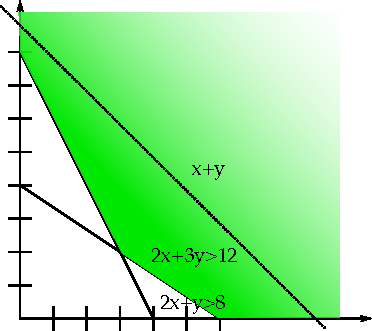
\includegraphics{./images/graphSolutionEx.pdf}
\end{minipage}
\hfill
\begin{minipage}[hbt]{0.4\linewidth}
\begin{align*}
\min x+y\\
2x+y\geq 8\\
2x+3y\geq 12
\end{align*}
\end{minipage}
\caption{An example for a graphical solution of an LP. The optimal solution is (3,2)}
\label{Fig:graphSolutionEx}
\end{figure}

How can we derive an algorithm from this method? We use the idea of sliding down, but just look at the corners of the feasible region, to get discrete steps (continuous sliding can't be implemented well). We start with any corner of the feasible region (a basic feasible solution) and look at its neighbors. Should they have a better objective value we move, else we're finished. 

To formalize the intuition from the 2D-space we need a notion of a corner in a (usually high dimensional) feasible region. To use it in a algorithm it should be a non-graphical definition. First we give some general definitions and then three different alternative definitions of a corner. We finish by proving that they are all equivalent.

\begin{Def}[Polyhedron] A set in $\R^n$ whose members obey a set of linear inequalities
\[\{x\in \R^n | Ax \geq b\} \qquad A\in \R^{m\times n},\ b\in \R^m\]
\end{Def}

\begin{Def}[Hyperplane, Hyperspace] \label{Def:hyperPlaneSpace} Let $a,x\in \R^n$, $a\neq 0$. 
\begin{enumerate}
\item $\{x|ax=b\}$ is a \emph{hyperplane} (a line in 2D)
\item $\{x|ax\geq b\}$ is a \emph{halfspace} (halfplane in 2D)
\end{enumerate}
\end{Def}

With definition \ref{Def:hyperPlaneSpace} we can say that a polyhedron is an intersection of a bunch of halfspaces.

\begin{Def}[Convex Sets] A subset $S \subseteq \R^n$ is called \emph{convex} if any convex combination between two points (graphically: points on a line between those points) is contained in the set. See figure \ref{Fig:convexNotConvex}
\[\forall \lambda \in [0,1], \forall x,y\in S: \lambda x + (1-\lambda) y \in S\]
\end{Def}

\begin{figure}[hbt]
\begin{center}
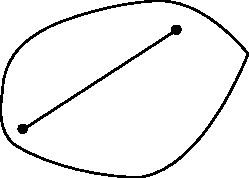
\includegraphics{./images/convex.pdf}\hspace{2cm}
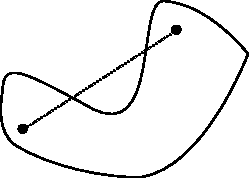
\includegraphics{./images/notConvex.pdf}
\end{center}
\caption{Graphical example for a convex and a non convex set (with non linear borders)}
\label{Fig:convexNotConvex}
\end{figure}

Convex sets have a lot of nice properties. Luckily feasible regions are always convex. This is the main reason why we can efficiently solve LPs. 

\subsection*{Corners}
The following three definitions formalize the notion of a corner.

\begin{Def}[Vertex]\label{Def:Vertex} Let P be a polyhedron. A vector $x\in P$ is a \emph{vertex} of P if $\exists \vec c\in \R^n$
 s.t. $cx < cy$ for all $y\in P, y \neq x $; that is $x$ is the minimal point for some cost vector (the unique optimal solution for some LP with the feasible set P). See figure \ref{Fig:vertex}
\end{Def}

\begin{figure}[hbt]
\begin{center}
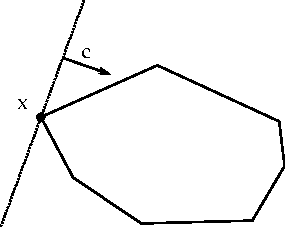
\includegraphics{./images/vertex.pdf}
\end{center}
\caption{A vertex $x$ is the optimal solution for a cost vector $c$}
\label{Fig:vertex}
\end{figure}

\begin{Def}[Extreme Point]\label{Def:ExtremePoint} An \emph{extreme point} of a polyhedron P is a vector $x\in P$ s.t. $x$ is not a convex combination of any two vectors $y,z\in P$ different from $x$. 
\end{Def}
Example: In 2D we can always select the two adjacent corners of a point $x$ on the edge of $P$ iff $x$ is not a corner. Then $x$ will be on the line between the two corners. 

\begin{Def}[Active Constraint]\label{Def:ActiveConstraint} Let $P$ be a polyhedron that is defined by some linear inequalities $a_i$: $P=\{x|a_ix\geq b_i\}$. We'll say that the $i$-th constraint is \emph{active} at a point $x$ if we have equality there $a_ix = b_i$
\end{Def}

\begin{Def}[Basic Feasible Solution]\label{Def:BFS} Let $P$ be a polyhedron in $n$ dimensions. Then $x\in P$ is a \emph{basic feasible solution} if the set of active constraints has full rank, that is there are $n$ linearly independent active constraint vectors at the point $x$. See figure \ref{Fig:bfsActiveConstraints}
\[\mbox{rank}(\{a_i\in \R^n|a_ix=b_i\}) = n\]

In particular there never is a b.f.s. if we have less than $n$ constraints. (Example: A line in 2D-Space or a plane in 3D-Space)
\end{Def}

\begin{figure}[hbt]
\begin{center}
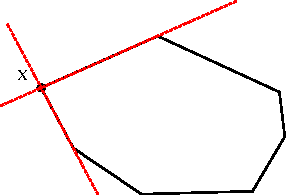
\includegraphics{./images/bfs.pdf}
\end{center}
\caption{Two constraints (red lines) are active at $x$. It's a basic feasible solution}
\label{Fig:bfsActiveConstraints}
\end{figure}

Now we want to prove that the three definitions \ref{Def:Vertex}, \ref{Def:ExtremePoint} and \ref{Def:BFS} are all equivalent to each other.

\begin{thm} \label{Thm:cornerEquiv} Let $P$ be a polyhedron and $x\in P$. The following are equivalent
\begin{enumerate}
\item $x$ is a vertex
\item $x$ is an extreme point
\item $x$ is a basic feasible solution
\end{enumerate}
\end{thm}

\begin{pr}[Theorem \ref{Thm:cornerEquiv}] The proof goes in three steps
\begin{itemize}
\item vertex $\Rightarrow$ extreme point: Proof by contraposition. Assume the existence of $y,z \in P$ s.t. $y,z\neq x$ with $x= \lambda y + (1-\lambda )z$. That is, $x$ is not an extreme point (definition \ref{Def:ExtremePoint}). We want to show that it's not a vertex either.

From definition a vertex (def. \ref{Def:Vertex}) we know that some $c$ should exist such that $c x < c \lambda y  + c (1-\lambda) z$. That however is a contradiction to the assumption $x= \lambda y + (1-\lambda )z$.
\begin{align*}
cx &= \lambda cy +(1-\lambda)cz\\
   &< \lambda cx + (1-\lambda)cx\\
   &< cx
\end{align*}

\item extreme point $\Rightarrow$ bsf (proof by contraposition; we show $\neg \text{bsf} \Rightarrow \neg \text{extreme point}$): Suppose $x\in P$ is not a basic feasible solution. Let $B$ be a matrix of active constraints at $x$ and $C$ the matrix of the inactive constraints such that $Bx=d$, $Cx\gneq f$ and $A = \left[B\atop C\right]$. Since $x$ is not a bfs the matrix $B$ hasn't full rank and its kernel is nonempty. Hence

\[\exists \delta \in \R^n, \delta \neq 0:\ B\delta =0\]

See figure \ref{Fig:extremeBfs}. With $\delta$ we define two vectors:

\[y=x+\epsilon \delta \quad z = x-\epsilon \delta\]

Note that $x=(z+y)/2$. That means that $x$ is not an extreme point if $z,y \in P$, because $x$ is a convex combination of the two. Consider 

\[Bz = B(x+\epsilon \delta) = Bx + \epsilon B\delta = Bx\]

Since $B\delta = 0$ the active constraints are still active. For the inactive constraints we have some slack before we leave the polyhedron (We can move around on the red line in figure \ref{Fig:extremeBfs}). If we choose $\epsilon$ small enough we're still within. It suffices to choose $\epsilon$ such that 

\[\forall i: \epsilon |c_i z| < c_i x - f_i\qquad \vec c_i\in C,\ f_i \in \vec f\]

Hence $z$ (and analogous $y$) are still in the polyhedron and $x$ is not an extreme point.

\begin{figure}
\begin{center}
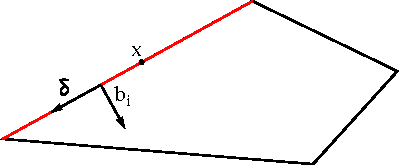
\includegraphics{./images/extreme_bfs.pdf}
\end{center}
\caption{$x$, active constraint $b_i$ and orthogonal vector $\delta$}
\label{Fig:extremeBfs}
\end{figure}

\item bfs $\Rightarrow$ vertex: Suppose $x$ is a bsf. Let $I$ be the indices of all active constraints and $c=\sum_{i \in I} a_i$. Then $c x = \sum_{i \in I} b_i$, since for each $a_i x \geq b_i $ the inequality is tight (see def. \ref{Def:ActiveConstraint}). 

Also $\forall y\in P, i\in I$ we have $a_i y \geq b_i$. Therefore $c y \geq c x$. The greater then is sharp as $x$ is the unique solution to the active constraints because it's a bfs and the system of active constraints has full rank, i.e. if n-lines cross in n-dimensional space they do so at \emph{one} point. (Theorem 2.2 in the Linear Optimization book). So $x$ is the optimal solution for some LP and hence a vertex.
\end{itemize}

\subsection*{Standard Form}
A LP in standard form\footnote{Cormen et al. name this slack-form (Schlupfform)} is of the form:
\begin{eqnarray*}
\text{minimize:}& \vec c \cdot \vec x \\
\text{subject to:} & A \cdot \vec x = \vec b \\
& x\geq0
\end{eqnarray*}

Any LP can be transformed into an equivalent LP in standard form. Two steps are needed for this, one to add non negativity constraints for all variables and a second to transform any inequalities into a equalities.

\paragraph*{Add non negativity constraints:} Suppose a variable $x$ has no non-negativity constraint. $x$ can be replaced with two variables $x'$ and $x''$ such that $x=x'-x''$ and $x',x''\geq 0$, as any negative number can be written as a combination of two non negative numbers.

\paragraph*{Remove inequalities:} Suppose a constraint $a$ to be $x_1+2x_2 \geq 15$. By adding a new variable $s\in \R$ and the constraint $a-s=15$ we can remove the inequality. So by adding a new vector $s\in \R^n$ with $A \cdot \vec x - s = \vec b$ the inequalities can be removed.

\end{pr}

\marginpar{Lecture 3}
To get a better intuition for the different definitions of a corner, we'll use them for some things that are not directly related to solving LPs.

\subsection*{Convex Hulls}

\begin{Def}(Convex Hull) Let $x_1,\ldots,x_k$ be some vectors in $\R^n$. The convex hull of these vectors is
\[\mbox{CH}(\{x_1,\ldots,x_k\}) = \left\{\sum _{i=1}^k \lambda_i x_i \left| \sum_{i=1}^k \lambda_i =1,\ \lambda_i\geq 0\right.\right\}\]
\end{Def}

Here we generalise the notion of convex combination to use more than two points. Intuitively if we have a bunch of points in 2D we get all the points that lie within the polygon that is spanned by the points on the CH, see figure \ref{Fig:convexHull}.

\begin{figure}[hbt]
\begin{center}
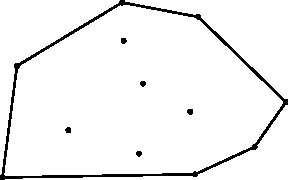
\includegraphics{./images/convex_hull.pdf}
\end{center}
\caption{The convex hull of a set of points}
\label{Fig:convexHull}
\end{figure}

This definition allows us to come up with a different definition of a polyhedron. In contrast to definition \ref{Def:polyhedron} the convex hull definition allows us to have a more geometric view of the problem.

\begin{Def}[Bounded Polyhedra] A bounded polyhedron lies within a finite bounding box, see figure \ref{Fig:bounded_unbounded}. More formally

\[\forall x\in P,d\in \R^n, \forall \lambda > 0: x+\lambda d \not \in P\]

For any line from a point inside the polyhedron we eventually leave the polyhedron
\end{Def}

\begin{figure}[hbt]
\begin{center}
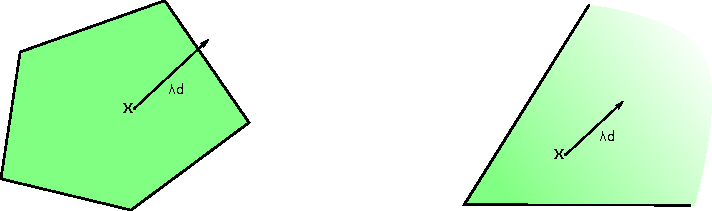
\includegraphics{./images/bounded_unbounded.pdf}
\end{center}
\caption{A bounded (left) and an unbounded (right) polyhedron}
\label{Fig:bounded_unbounded}
\end{figure}

\begin{thm}\label{Thm:CH_polyhedron} Let $P$ be a non-empty bounded polyhedron. Then $P=$\mbox{CH}(extreme points $P$)
\end{thm}

\begin{pr}[Theorem \ref{Thm:CH_polyhedron}] We prove equality by showing mutual inclusion:
\begin{description}
%#todo
%sieht unschoen aus, muessten wir anders formatieren
\item[$\text{CH(extreme points of P)} \subseteq \text{P}$] As polyhedra are convex sets. Every convex combination of extreme points must be in $P$.\\ 
\item[$\text{P} \subseteq \text{CH(extreme points of P)}$]:  From the definition we know that all convex combinations of two points are still in P. We generalise to the new kind of convex combination that includes several vectors. 

Let $x\in P$. Since $P$ is a polyhedron $x$ is a solution of the system of inequations $Ax\geq b$ (def. \ref{Def:polyhedron}). As in the proof for theorem \ref{Thm:cornerEquiv} we separate $A$ into the matrix $B$ of active constraint and $D$ of inactive constraints, with $Bx=d$, $Dx>f$. If the rank of $B$ is $n$, $x$ is an extreme point by definition and we're done. 

The other possibility is $\rank B=k$ and $k<n$. We use the same trick as in proof \ref{Thm:cornerEquiv} to find two new points. Since the matrix hasn't full rank, there has to be $\delta \neq 0$ such that $B\delta = 0$. As before we build two vectors $x_1 = x+ \epsilon_1 \delta$, $x_2=x-\epsilon_2 \delta$. 

Now we want to get from these points somehow to extreme points, as we want to prove that we can use extreme points to represent every point in $P$. We choose $\epsilon>0$ as the largest value such that $x_1$ is still a feasible solution, that is, we follow a line through $x$ until we reach a boundary of the polyhedron. See figure \ref{Fig:convCombExPoints} for a graphical representation of the process in a 2D-Polyhedron.

\begin{figure}[hbt]
\begin{center}
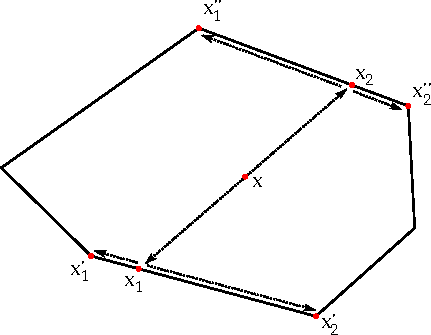
\includegraphics{./images/convex_comb_extr_points.pdf}
\end{center}
\caption{$x$ can be written as a convex combination of $x_1',x_2', x_1''$ and $x_2''$}
\label{Fig:convCombExPoints}
\end{figure}

Such an $\epsilon$ has to exist, since the polyhedron is bounded and therefore every line eventually crosses a boundary.\footnote{The calculation we did in the lecture to find $\epsilon_{1,2}$ seems dubious to the authors. We'll investigate.} Choosing $\epsilon$ like this implies that some constraint $a_i$ in $D$ has to become active for $x_1$ and the same holds with a different $a_i$ for $x_2$. Moving in direction $\delta$ doesn't affect the constraints that already were active, since $\delta$ is in the kernel of $B$. So we increase the number of active constraints and can extend $B$ to 

\[\begin{pmatrix}B\\ a_i\end{pmatrix}\] 

The rank of the new $B$ has to be $k+1$ since $\delta$ was orthogonal to all the vectors in $B$, as $B\delta=0$ (and hence all vectors in $\text{span } B$), but it is not orthogonal to $a_i$, or we wouldn't have hit that constraint by moving in direction $\delta$.

We have now reduced the problem of finding extreme points to represent $x \in P$ to the problem of finding some for $x_1,x_2 \in P$. However we increased the number of active constraints for $x_1,x_2$ (in 2D: we moved them on an edge). This process can be repeated for $x_1$ and $x_2$ until the respective $B$ has full rank and we arrived at some extreme points. For figure \ref{Thm:CH_polyhedron} the process is repeated three times, for $x,x_1$ and $x_2$. 
Since all the points from the beginning can be recursively written by a convex combination of the new points and we end up at an extreme point, the original $x$ can transitively be written by a convex combination of extreme points.
\end{description}

% Ich hab noch drüber nachgedacht und die Rechnung da in der Tat komisch zu sein. Er (oder ich :D) scheint sich zwischendurch verrechnet zu haben. Wir haben nicht genug info das zu lösen:
%
% x&=\lambda x_1+(1-\lambda)x_2 % ist die Linie zwischen x1,2 auf der x liegt. Wir wollen x_1,2 soweit nach außen schieben dass wir am Rand ankommen
% x&=\lambda (x+\epsilon_1\delta) + (1-\lambda)(x-\epsilon_2\delta) % ist das selbe nochmal neu geschrieben. Jetzt wollen wir nach den epsilons auflösen ???
% x-\lambda x - (1-\lambda) x = \lambda \epsilon_1\delta + (1-\lambda)\epsilon_2\delta
% x -\lambda x - x +\lambda x  = \epsilon_1\delta +\epsilon_2\delta
% 0 = \epsilon_1 \delta + \epsilon_2\delta
% ???
% Profit.



%In particular choose \label{wieso}
%\begin{align*}
%x&=\lambda x_1+(1-\lambda)x_2\\
%&=x+\underbrace{\lambda \epsilon_1\delta -(1-\lambda)\epsilon_2\delta}_{\stackrel{!}{=}0}\\
%&\Rightarrow \lambda = \frac{\epsilon_2}{\epsilon_1+\epsilon_2}
%\end{align*}

\end{pr}

\begin{cor}\label{Cor:always_extreme_points} Let $P$ be a non-empty bounded polyhedron. Then the LP $\min cx$ s.t. $x\in P$ always has an optimal solution that is an extreme point of $P$.
\end{cor}

Intuitively this is true, as given an optimal solution, which is not an extreme point, we could always go into the direction of a constraint which is not tight. Such a constraint must exist, as otherwise we would be at an extreme point. 

\begin{pr}[Corollary \ref{Cor:always_extreme_points}] %(from the book 'Linear Optimization') 
Start with some optimal solution $x^*$. Write it as a convex combination of extreme points 
\[x^* = \sum_{i=1}^x \lambda_i y_i \qquad \text{s.t. } y_i \text{ is an extreme point}\]
We want to prove that there is an extreme point $y_i$ such that the cost $v$ are the same as in $x^{*}$, that is:

\[v = cx^* = cy_i\]

Obviously $cy_i\geq v$ since $x^*$ is an optimal solution. It can't be strictly greater for all $y_i$ or 
\[c\sum_{i=1}^x \lambda_i y_i \gneq v\]
since the $\lambda_i$ are greater than zero and $\sum_i \lambda_i =1$. This would be a contradiction since $x^*=\sum_{i=1}^x \lambda_i y_i$. So there has to be at least one extreme point $y_i$ for which $cy_i=v$.
\end{pr}

Corollary \ref{Cor:always_extreme_points} gives us the nice result that we can transform the problem of optimising an LP to a discrete problem with finitely (albeit exponentially) many candidate solutions. This will of course be very useful in designing an algorithm for solving them.

\subsection*{Fourier-Motzkin elimination}

In this section we're interested in computing representations of projections of polyhedra. See figure \ref{Fig:polyhedron_proj} for an example.

\begin{figure}[hbt]
\begin{center}
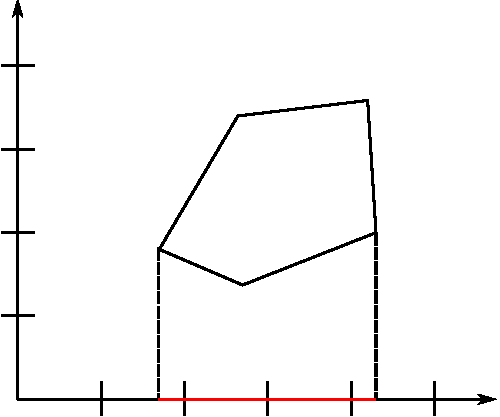
\includegraphics[width=0.3\textwidth]{./images/polyhedron_proj.pdf}
\end{center}
\caption{A projection which removes one of the two dimensions.}
\label{Fig:polyhedron_proj}
\end{figure}

\begin{Def} The projection $x=(\nthings{x})$ onto its first $k$ coordinates is $\pi_k(x) = (x_1,\ldots, x_k)$. 

Let $S\subseteq \R^n$ then the projection on the first $k$ components is

\[\pi_k(S)=\{\pi_k{x}|x\in S\}\]
\end{Def}

Of course that definition is not particularly useful in actually constructing the projection. The Fourier-Motzkin elimination computes the projection for polyhedra. We start with our usual characterisation of a polyhedron $P=\{x|Ax\geq b_i\}$ and want to find a different matrix $A'$ s.t. we get $\pi_{n-1}(P)$. Generalizing to $\pi_k$ is then of course easy.

\subsubsection*{Example of Fourier-Motzkin elimination}
Figure \ref{Fig:motzkinExample} shows an example of the Fourier-Motzkin elimination. The LP used for the example is:
\begin{eqnarray*}
c_1 & -0,5x + y & \leq 3 \\
c_2 & 2x + y & \leq 6 \\
c_3 & x+3y & \geq 6 \\
c_4 & x+y & \geq 2
\end{eqnarray*}
Those constraints can be rewritten to:
\begin{eqnarray*}
c_1 & \frac{1}{2}x + 3  & \geq y \\
c_2 & -2x+6 & \geq y \\
c_3 & y & \geq -\frac{1}{3}x+2 \\
c_4 & y & \geq -x+2
\end{eqnarray*}
Writting them this way has the advantage of ordering them around $y$. With this information we can build a new LP, which constraints are only on the x-dimension. The constraints are all the ordered pairs of around $y$.
\begin{eqnarray*}
c_1 \geq c_3: & \frac{1}{2}x + 3 & \geq -\frac{1}{3}x+2  \\
c_2 \geq c_3: & -2x+6 &  \geq -\frac{1}{3}x+2 \\
c_1 \geq c_4: & \frac{1}{2}x + 3   & \geq -\frac{1}{3}x+2 \\
c_2 \geq c_4: & -2x+6 & \geq -x+2
\end{eqnarray*}
Those constrains are shown in figure \ref{Fig:motzkinExample} below the x-axis with dashed lines. Note that we're only interested in the red part. So the two constraint $c_2 \geq c_3$ and $c_1 \geq c_4$ would be enough. As there is no efficent way to find those two constraints we have to keep all of them. 

\begin{figure}[hbt]
\begin{center}
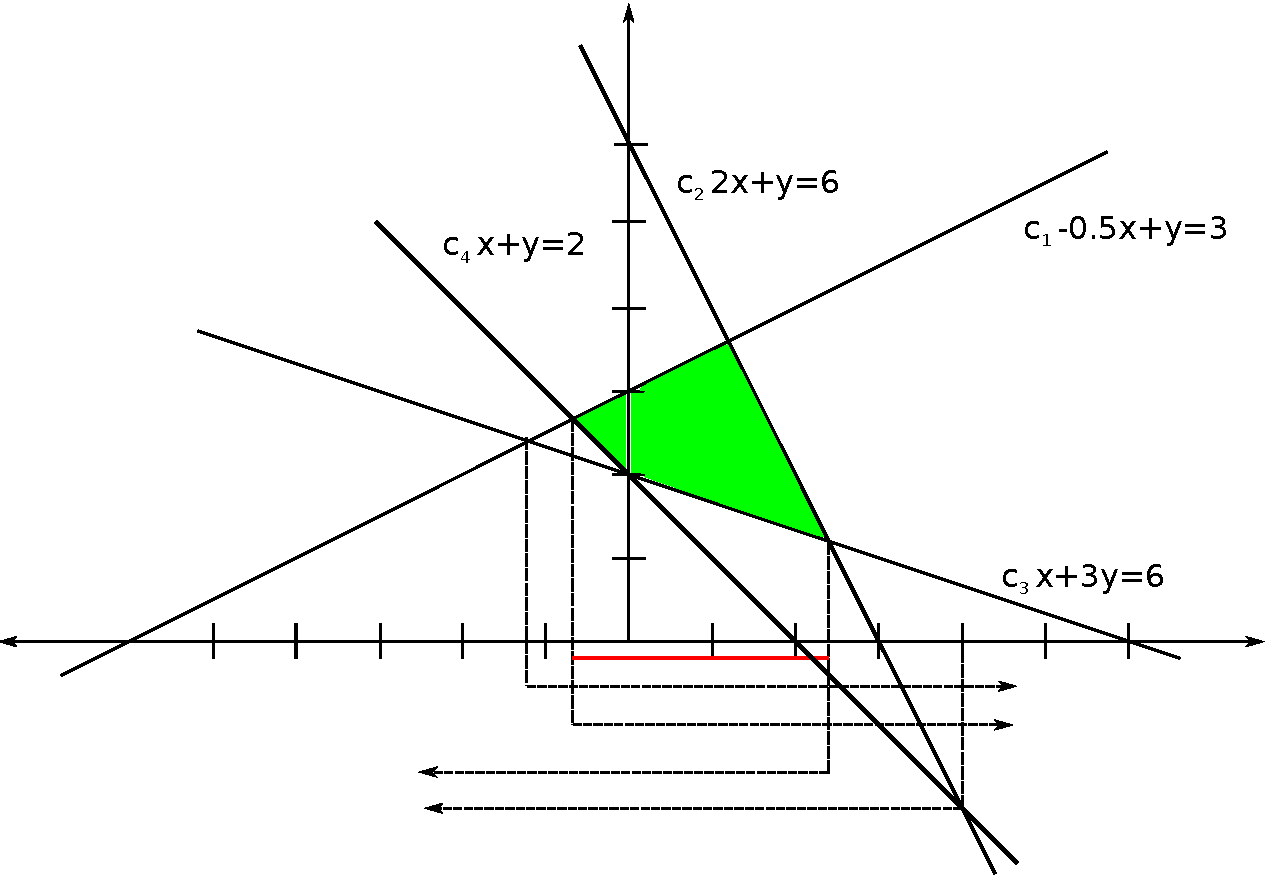
\includegraphics[width=0.8\textwidth]{./images/motzkin.pdf} %TODO die gestrichelten Linien mit c_1,..,4 beschriften 
\end{center}
\caption{A projection, which removes one of the two dimensions. The result is shown in red.}
\label{Fig:motzkinExample}
\end{figure}

\subsubsection*{General case}
We want to classify the constraints $a_i$ into three kinds. Let $\overline a = \pi_{n-1}(a)$ then we can write  

\[P=\left\{x\left| \begin{array}{cr}
\overline a_i\overline x +a_{in}x_n \geq b_i & i\in T_1\\
\overline a_i\overline x +a_{in}x_n \geq b_i & i\in T_2\\
\overline a_i\overline x \geq b_i & i\in T_3\\
\end{array}\right.\right\}\]

With 
$$\forall i\in T_1: a_{in}>0$$ $$\forall i\in T_2: a_{in}<0$$ $$ \forall i\in T_3: a_{in}=0 $$

From that form we rewrite the polyhedron by dividing with $\overline a_{in}$ if $\overline a_{in}\neq 0$. The $f_i$ are vectors and the $d_i$ are scalars. 

\begin{equation}\label{For:Motz1}x_n \geq  d_i + f_i \bar x : i \in T_1 \end{equation}
\begin{equation}\label{For:Motz2}x_n \leq  d_i+f_i \bar x : i \in T_2 \end{equation}
\begin{equation}\label{For:Motz3}0 \geq  d_i+f_i \bar x : i \in T_3 \end{equation}

%\[P \{i\in T_1 \wedge x_n \geq d_i + f_i \bar x \vee i\in T_2 \wedge x_n \leq d_i + f_i \bar x \vee i\in T_3 \wedge 0 \leq d_i + f_i \bar x\}\]

Then we can write the projection $\overline P=Q$ as\footnote{Adrians lecture notes as well as mine read: $\{d_i+f_i\bar x \leq d_j+f_j\bar x\ \forall i\in T_2, j\in T_1 $. The book says $\geq$ and $T_2\geq x_n \geq T_1$}

\begin{eqnarray*}
\{d_i+f_i\bar x & \geq d_j+f_j\bar x\ & \forall i\in T_2, j\in T_1  \\
d_i+f_i\bar x & \geq 0\ & \forall i\in T_3\}
\end{eqnarray*}

%$$\{d_i+f_i\bar x \geq d_j+f_j\bar x\ \forall i\in T_2, j\in T_1 $$ 
%$$d_i+f_i\bar x \geq 0\ \forall i\in T_3\}$$

Herein lies the problem of the algorithm. We introduce a new constraint for every pair of constraints from $T_1,T_2$. Hence in every iteration the number of constraints $c$ can grow on the order of $(\frac{c}{2})^2$.

\subsubsection*{Proof of correctness}
\begin{pr} To prove the correctness of the Fourier-Motzkin elimination we need to show that the result $Q$ of the algorithm is equal to $\pi_{n-1}(P)$. We do this by showing $\pi_{n-1}(P) \subset Q$ and $Q \subset \pi_{n-1}(P)$.
\begin{enumerate}

\item $\bar x \in \pi_{n-1}(P) \Rightarrow \bar x\in Q$. That means 
\[\exists x_n: \left[{\bar x}\atop{x_n}\right] \in P \Rightarrow {{\max_{i\in T_1} d_i +f_i \bar x \leq x_n} \atop {\min_{i\in T_2} d_i+fi\bar x \geq x_n}}\]
Therefore the constraints \ref{For:Motz1}, \ref{For:Motz2} and \ref{For:Motz3} are satisfied. It follows that $\bar x \in Q$. 

\item $\bar x \in Q \Rightarrow \bar x \in \pi_{n-1}(P)$. Choosing $x_n$ as 
\[x_n \in [\max_{i\in T_1} d_i+f_i \bar x, \min_{i\in T_2} d_i+f_i \bar x]\]
does the trick, as $(\bar x, x)$ then satisfies constrains \ref{For:Motz1}, \ref{For:Motz2} and \ref{For:Motz3} and therefore is in $P$.

\end{enumerate}
\end{pr}

There are a lot of interesting applications for these projections:

\begin{thm}\label{Thm:linTransPoly} Let $P\in \R^n$ be a polyhedron and $A\in \R^{m\times n}$ be a matrix. Then the set
\[Q=\{Ax|x\in P\}\]
is also a polyhedron.
\end{thm}

In 2D this is intuitively clear: applying linear transformations on polygons results in distorted, rotated etc. polygons. For higher dimensions it follows from the projections:

\begin{pr}[Theorem \ref{Thm:linTransPoly}] For $P$ we have

\[Q=\{(Ax,x)\in \R^{m+n}| x\in P, P\text{ is a polyhedron in } \R^{n}, A \in \R^{m \times n}\}\]  %this is actually not that intuitive for me. Why is this a polyhedron?

is a polyhedron. Then $\pi_m(Q)$ is also a polyhedron.
\end{pr}

\begin{cor} Let $x_1,x_2,\ldots, x_k \in \R^n$, then CH($x_1,x_2,\ldots, x_k$) is a polyhedron\end{cor}

\paragraph*{Optimal value} We can use the projections to find the optimal value for an LP (not the optimal solution though). Suppose we're given a LP in the usual form, $\min cx$ s.t. $Ax\geq b$. We construct the following polyhedron P:

\begin{eqnarray*}
 & (x_0,\ldots,x_n) & \\
s.t. & A(x_0,\ldots,x_n)^{\mbox{T}} & \geq b \\
& c(x_0,\ldots,x_n)^{\mbox{T}} & = x_0
\end{eqnarray*}

Define $Q = \pi_1(P)$. We can find $Q$ with the Fourier-Motzkin elimination. If $Q$ is not feasible, $P$ is empty. Else we can choose the biggest $b_i$ such that $x_0\geq b_i$ or the smallest $b_i$ such that $x_0 \leq b_i$, depending on the type of constraints we have. That is the optimal value.

\begin{thm}[Farkas' lemma] Let $A\in \R^{m\times n}$ and $b\in \R^m$. Then either 
\begin{itemize}
\item $\exists x\in \R^n: Ax\geq b$ or
\item $\exists y\in \R^m, y\geq 0, y^{\mbox{T}}A=0: y\cdot b>0$
\end{itemize}
\end{thm} 

This theorem is very nice if we want to check if some system of inequalities is feasible. We just have to find the vector $y$. This lemma can be proven by our earlier results. (Sketch:) We start with the polygon $P$ and use a projection to get rid of the last dimension of $P$. By that we get another matrix $B$ and another vector $d$. We get the new inequalities by combining those from the original polyhedron. Instead of actually doing the projection to a lower dimension we can replace the last element by 0. You can show that $[B0]=DA$ (no proof). You can repeat that process until you get a matrix $F$ such that $FA=0$. The system is infeasible if you end up with a negative rhs for a constraint, since all lhs will be 0.

\marginpar{Lecture 4}
\subsection{The simplex algorithm}
Recall that an LP is in standard form if

\begin{align*}
\min cx\\
Ax = b\\
x\geq 0
\end{align*}

and $A\in \R^{m\times n}$ has $m$ linearly independet rows. A basis $B\subseteq [1,n]$ is as set of $m$ indices such that $A_B$ has full rank $m$. It induces a basic solution

\[\begin{cases} x_B = A^{-1}_Bb\\ x_{\bar B} = 0\end{cases}\]

We say it is feasible if $x_B\geq 0$. Note that the $x_{\bar B}=0$ part makes $n-m$ non-negativity constraints active so that we actually are at a corner with $n$ active constraints in $n$ dimensions.

The simplex algorithm works by moving from corner to corner, always in the direction of better costs. At first we'll have some simplifying assumptions, to avoid the messy details:

\begin{enumerate}
\item The LP is in standard form (for conversion see \ref{Sec:standardForm})
\item Every feasible basis $A$ is non-degenerate. A basis $B$ is non-degenerate if $\forall b:\ x_B=A^{-1}_Bb \gneq 0$. Note the difference to $x_B\geq 0$ for general basic solutions. So it is forbidden that more than $n$ (those in $B$ and $>n-m$ non-negativity) constraints are active (in $n$ dimensions they can't all be linearly independet of course). 
\item We are given an initial feasible basis
\item The feasible region of the LP is bounded
\end{enumerate}

In the next lectures we'll remove those assumptions one after the other.

The algorithm works as follows:
\begin{lstlisting}
SIMPLEX-TAKE-I(A,b,c)

B <- find some feasible basis
// B=$\{b_1,b_2,\ldots, b_m\} \subseteq [1,\ldots, n]$
repeat 
    for $j\in [1,n]\backslash B$ and  $b_i \in B$
        D = B $\cup$ j $\backslash$ $b_i$
        if D is a basis then
            $x_B$ = $A^{-1}_B$b
            $y_D$ = $A_D^{-1}b$ // a bfs
            if ($y_D$ $\geq$ 0 and $c_Dy_D < c_Bx_B$)
                B = D
until B hasn't changed                
\end{lstlisting}

$D$ is build by removing one constraint from $B$ and adding another one that wasn't in there before. We then check if $D$ is non-singular. If so it induces a basic solution, we just have to check if it's feasible. If yes we check if the cost improves and move to $D$ if it does.

It will later turn out that we don't actually have to check every combination for $j$ and $b_i$. The choice of $b_i$ is uniquely determined.

We can't get the same basic solution from two different bases, if we have a non-degenerate LP. In the degenerate case this may very well happen:

\begin{align*}
x_2 + x_3 &= 1\\
x_1 - x_2 +x_4 &=0\\
x_1 + x_2 +x_5 &= 2\\
\end{align*}

% figure

The above system gives us the solution $(1,1,0,0,0)$ for three bases $\{1,2,3\},\{1,2,4\},\{1,2,5\}$. This happens because we have a point where three constraints are active, although we're in 2D. See figure \ref{Fig:degenerateLP}. It is easy to see that if we have two bases build from indices $k\in [1,\ldots,n]$ that give us the same solution one of the $x_k$ (a basic variable) has to be zero. %easy to see :S

%figure

We move from solution $x$ to solution $y$ along some vector $d$ ($y=x+\Theta d$). Have a look at figure \ref{Fig:movingToSolutions}. We do some observations on the vector $d$. 

\begin{itemize}
\item $d_k=0$ if $k\not \in B \cup j$, because we assumed all variables not in the basis (i.e. the non-basic variables) to be zero to make the non-negativity constraints active 
\item $d_j>0$ $(x_k=0, y_k=0)$. By choosing $\Theta$ accordingly we can scale this to be $d_j=1$
\item $Ad = 0$ ($Ad = (Ay-Ax)/\Theta = (b-b)/\Theta = 0)$
\end{itemize}

By using these observations we can directly calculate the $b_i$ we need to remove.

We can rewrite $A_d$ like follows and can use that to find the components of $d$:

\[A_d = A_B d_B+A_j = 0 \Rightarrow d_B = -A^{-1}_B A_j\]

We also want $y\geq 0$ so that we need

\[x_B - d_B = x_B - \Theta A_B^{-1} A_j \geq 0\]

Thet means if $d_{b_i}>0$ we are ok, however if $d_{b_i} <0$ then $x_{b_i} +\Theta_{b_i} \stackrel{!}{\geq} 0$ so $\Theta \leq \frac{-x_{b_i}}{d_{b_i}}$. We can do that by choosing

\[\Theta = \min_{{b_i\in B}\atop {d_{b_i} <0}} \left| \frac{x_{b_i}}{d_{b_i}}\right |\]

So the indices attaining the minimum will be the ones we'll have to take out. Because we assumed that the system is non degenerate there will be only one element actually attaining it. %why does non-degenerate imply that?

How does the cost change?

\[cy -cx = \Theta cd = \Theta(c_j+c_Bd_B) = \Theta(c_j - c_B^TA^{-1}_B A_j)\]

If $y$ was a solution that we move to we did that because $cy$ was smaller that $cx$. So $c_j - c_B^TA^{-1}_B A_j$ should be negative if we want to move to $y$

\begin{lstlisting}
SIMPLEX-TAKE-II (A,b,c)

B = some feasible basis
repeat 
    for $j\in \{1,\ldots,n\}\backslash B$ // $b_i$ is determined
        $d_B$ = $A^{-1}_B A_j$
        if $c_j - c_B^TA^{-1}_B A_j < 0$
            $b_i$ = index  s.t. $d_{b_i} <0$, 
                    minimizing $\left| \frac{x_{b_i}}{d_{b_i}}\right|$
            B = B $\cup$ j $\backslash$ $b_i$
until B hasn't changed
\end{lstlisting}

%todo rechnungen zwischen II und III

\begin{lstlisting}
SIMPLEX-TAKE-III (A,b,c)

B = some feasible solution
repeat
    $\bar c$ = c - $c^T_B A^{-1}_BA$ //reduced cost vector
    if $\exists j:{\bar c}_j<0$ 
        u = $A^{-1}_B A_j$ // dimension m
        $b_i$ = index in B s.t. $u_i >0$ 
                minimizes  $x_{b_i}/u_i$
        B = B $\cup$ j $\backslash b_i$ 
until B hasn't changed 
// $\bar c \geq 0$ 
\end{lstlisting}

The algorithm always terminates because the assumptions ensure that we always have a optimal solution and we improve our solution in every step.

\begin{thm}\label{Pr:simplexIIIopt} Let B be a basis. If $x_B=A^{-1}_Bb\geq 0$ and $\bar c=c-c_B^{T}A_B^{-1}A_j$ then $B$ is optimal.\end{thm}

\begin{pr}[Theorem \ref{Pr:simplexIIIopt}] Let $x$ be the bsf induced by $B$, $y$ be some feasible solution. We want to argue that the cost of $x$ is smaller than the cost of $y$. Let $d=y-x$ then 
\[cd = c_Bd_B + \sum_{j\in \bar B} c_jd_j \] 

To be continued
\end{pr}
\end{document}
